% !TeX document-id = {38ad272c-6b95-4178-b409-8ae7f3766667}
% !TeX spellcheck = en_US
% !TeX root = ../../build/architecture.tex
% !TeX TXS-program:compile = txs:///xelatex/[--shell-escape]


\renewcommand{\mytitle}{The Road to Ethereum Scalability}
\ifZEROSEC \fi
\ifSEC \section{\mytitle{}}\fi
\ifSUBSEC \subsection{\mytitle{}}\fi
\ifSUBSUBSEC \subsubsection{\mytitle{}}\fi


\begin{frame} {Scaling Blockchain and the Scaling Trilemma}
\begin{block}{Scaling Blockchain}
When we talk about scaling blockchain, we talk about \textbf{increasing the number of processed transactions per second}.
\end{block}
\begin{itemize}
\item The term \textbf{scalability trilemma} was first coined by \textit{Vitalik Buterin} to describe the inherent tension between three properties that a high-performing blockchain platform must have:
  \begin{enumerate}
  \item Decentralization.
  \item Security.
  \item Scalability.
  \end{enumerate}
\item The trilemma refers to the belief that blockchain platforms can only achieve two of these three goals effectively.
\end{itemize}
\end{frame}



\begin{frame} {How to scale?}
  \textbf{Approach \#1}
  \begin{itemize}
    \item Increase transactions per block.
    \item This may lead many blockchain nodes to exhaust their resources.
    \item Therefore, this may trigger centralization (a network with only powerful nodes).
  \end{itemize}
  \textbf{Approach \#2}
  \begin{itemize}
    \item Do \textbf{sharding}, which means split the burden in shards.

    \item A node only deals with a \textit{portion} of the burden, i.e. with the operations
    in its shard.

    \item There are several approaches within the sharding strategy.
  \end{itemize}
\end{frame}






\begin{frame} {Approach \#2.a: Sharding for Data Availability and Execution}
  \begin{itemize}
    \item The first approach consists in using the current L1 chain as a \textit{consolidation chain}, 
    which will be renamed as the L1 \textbf{beacon chain}.
    \item Then, use \textbf{availability} and \textbf{execution} in each shard:

    \begin{figure}
      \centering
      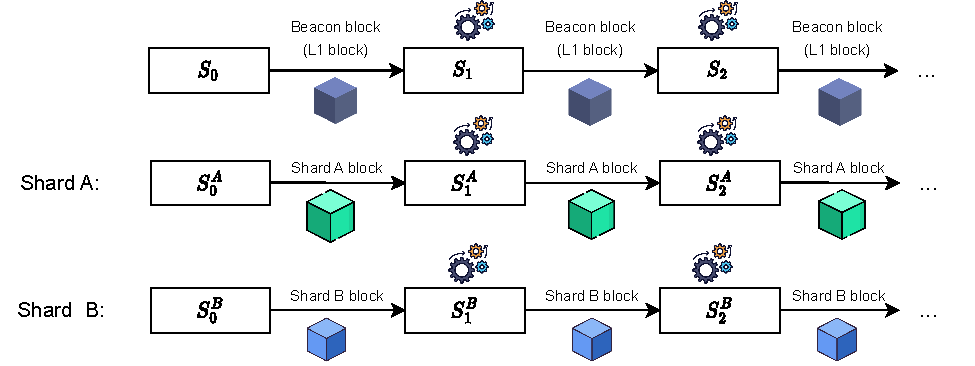
\includegraphics[width=0.9\columnwidth]{\zkevmdir/figures/concepts/road-to-scalability/execution-shard-chains.drawio}
    \end{figure}
  \end{itemize}
\end{frame}





\begin{frame} {Problems of Sharding with Data\_Availability+Execution}
The previous approach is a L1 design with \textbf{availability and execution} in each shard.

\vspace{0.15cm}
However, this produces a huge instability in Ethereum L1 specifications:
\begin{itemize}
\item L1 Ethereum is responsible for the managements of each of shard's states.
\item This includes the \textbf{execution} and \textbf{inter-shard messaging} when necessary.
\item This does not allow L1 \textbf{ossification}.
\end{itemize}
\end{frame}





\begin{frame}{Approach \#2.b: Data Availability Sharding and a Single Execution Layer}
\begin{itemize}
\item In this approach Ethereum specifications provide:
  \begin{enumerate}
  \item Just \textbf{ONE L1 execution layer} giving execution and availability (that is, the current L1).
  \item Data availability sharding scheme (\href{https://ethereum.org/ca/roadmap/danksharding}{danksharding}).
  \end{enumerate}
\begin{figure}
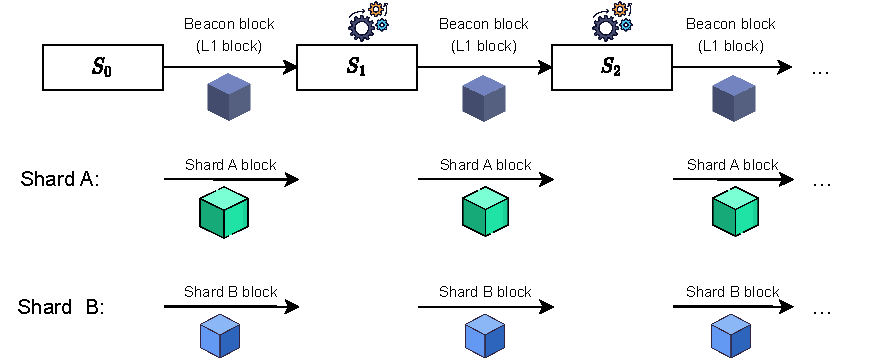
\includegraphics[width=0.8\columnwidth]{\zkevmdir/figures/concepts/road-to-scalability/data-shard-chains.drawio}
\end{figure}
\end{itemize}
\end{frame}




\begin{frame}{\texttt{blobs}}
\begin{columns}
\begin{column}{0.4\textwidth}
Instead of transactions, shard blocks contain \textbf{blobs} (binary large objects) that designed to be interpreted by a top layer.
\end{column}
\begin{column}{0.58\textwidth}
\begin{figure}
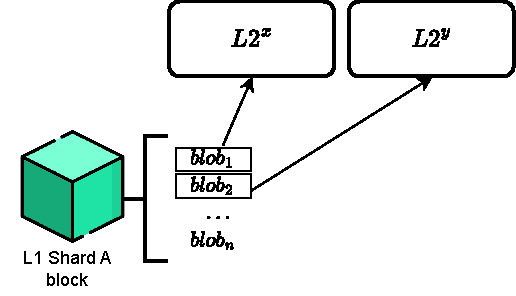
\includegraphics[width=0.8\columnwidth]{\zkevmdir/figures/concepts/road-to-scalability/block-of-blobs.drawio}
\end{figure}
\end{column}
\end{columns}
\end{frame}




\begin{frame}{L2 Layers}
\begin{itemize}
\item New top layers, called \textbf{L2 layers}, can be created on top of this L1 machinery.
\item L2's define how they manage the state: 
  \begin{itemize}
  \item A payment system with simple transactions.
  \item A token transfer system.
  \item A system with smart contracts.
  \end{itemize}
\item L2's also define how they use L1:
  \begin{itemize}
  \item The L1 execution layer.
  \item The data shards (when available\footnote{Regarding the current situation of data sharding,
  L1 data shards specification is still under develop (the \textbf{EIP 4484} is currently on the "review stage"). 
  For this reason, currently, all the scaling solutions use the availability of the execution layer.}).
  \end{itemize}
\end{itemize}
\end{frame}





\begin{frame}{Building a Layer 2}
\begin{columns}
\begin{column}{0.35\textwidth}
\begin{itemize}
\item Let's assume that our layer 2 is called x ($L2_x$).
\item The state of the layer x progresses with its L2 transactions.
\end{itemize}
\end{column}
\begin{column}{0.65\textwidth}
\begin{figure}
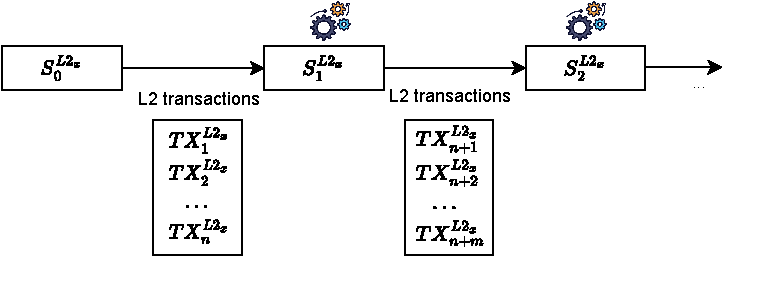
\includegraphics[width=\columnwidth]{\zkevmdir/figures/concepts/road-to-scalability/l2-state.drawio}
\end{figure}
\end{column}
\end{columns}

\begin{itemize}
\item There are many questions to answer to build an L2:
  \begin{enumerate}[a)]
  \item How users send L2 transactions and who receives them?
  \item How these L2 transactions are made publicly available (if so)?
  \item Who processes the L2 transactions and how, and, when 
  it is publicly considered that a new state is correctly computed?
  \item What type of applications the L2 supports? simple or rich processing?
  \end{enumerate}
\end{itemize}
\end{frame}